\section{Introduction}

\subsection{The {\nbody} problem}
\begin{frame}
    \frametitle{The {\nbody} problem}
    \framesubtitle{Definition (1/2)}

    \begin{columns}
        \begin{column}{0.6\textwidth}
                \begin{block}{}
            \begin{center}
                Predicting motion of a group or celestial objects that interact
                each other gravitationally.
            \end{center}
            \end{block}
        \end{column}
        \begin{column}{0.4\textwidth}
        \begin{figure}
            \centering
            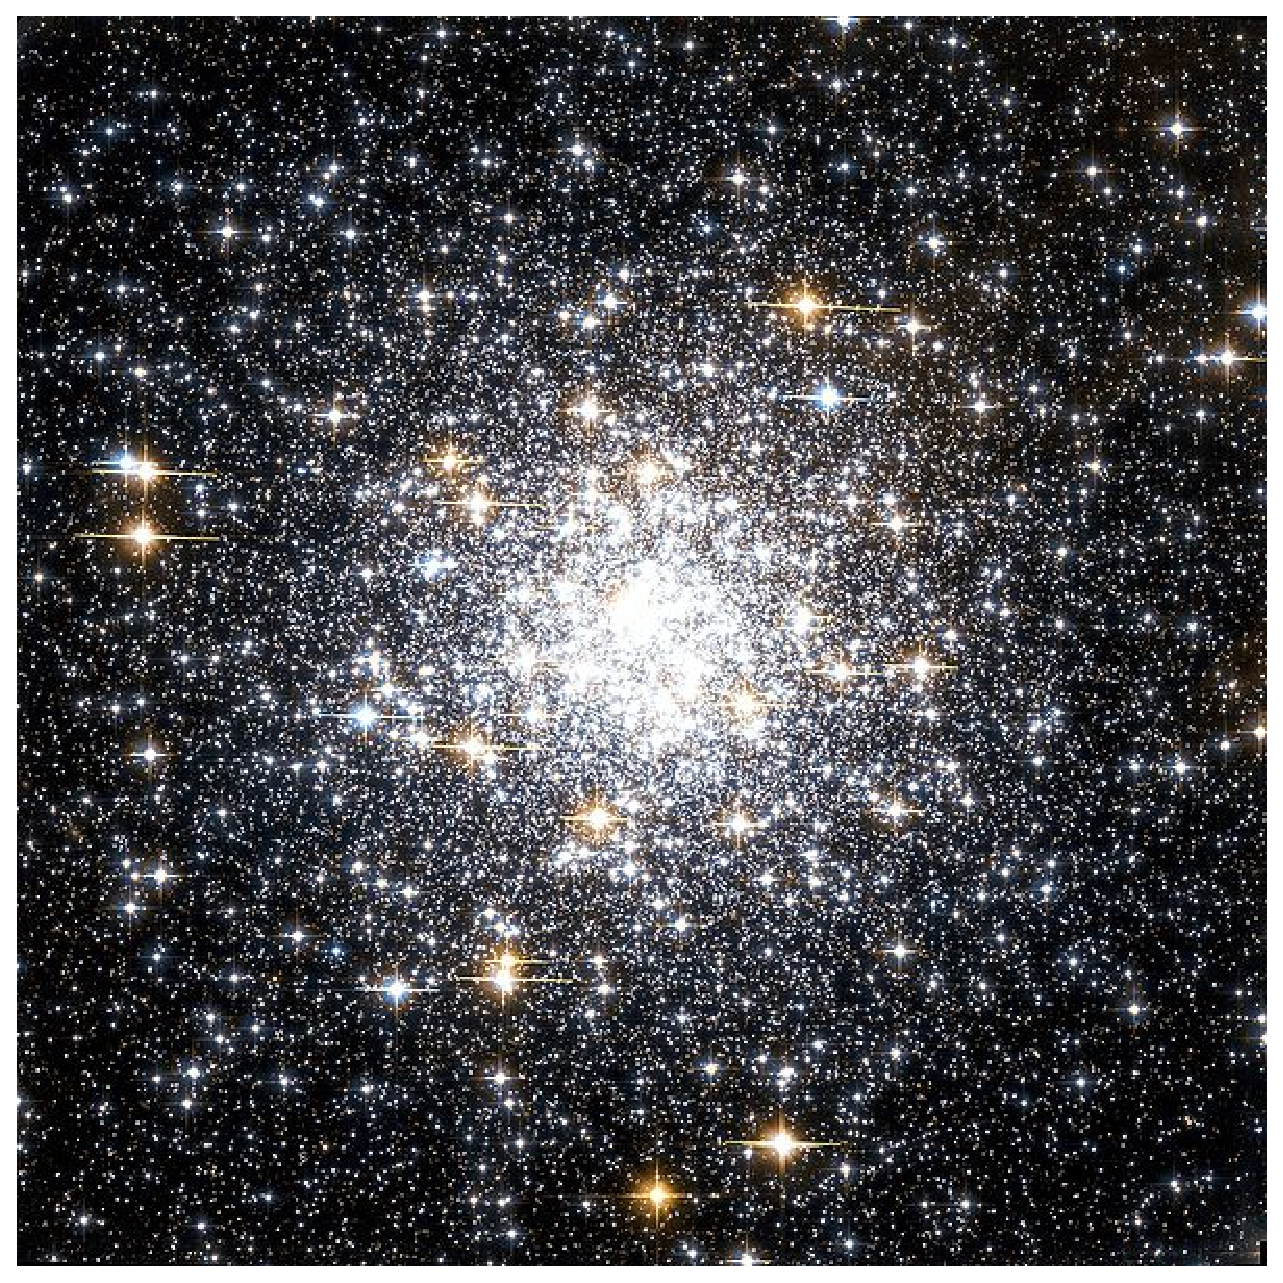
\includegraphics[width=0.8\textwidth]{img/m69}
            \caption{M69 in Sagittarius.}
            \label{fig:m69}
        \end{figure}
        \end{column}
    \end{columns}

\end{frame}

\begin{frame}
    \frametitle{The {\nbody} problem}
    \framesubtitle{Definition (2/2)}

    Purely dynamic problem, in which the bodies orbital evolution
    is determined exclusive by the \blue{gravitational interaction},

    \begin{align}
        \ddot{\vec{r}}_{i} &= -G \sum\limits^{N}_{\substack{j=1\\j\neq i}}
                              m_{j}\ \dfrac{\vec{r}_{ij}}{
                              | \vec{r}_{ij}|^{3}}\label{eq:nbody},
    \end{align}

    \noindent
    where \soft{$G$} is the gravitational constant,
%    ($6.67384\times 10^{-11} m^{3} kg^{-1} s^{-2}$),
    \soft{$m_j$} is the mass of the \soft{$j-$}th particle
    and \soft{$\vec{r}_{ij} = (\vec{r}_i - \vec{r}_j)$} the position in \emph{Cartesian} coordinates.
    %\begin{block}{\red{Note}}
    %    We denote vectors by \textbf{bold\ fonts}.
    %\end{block}
\end{frame}


\begin{frame}
    \frametitle{The {\nbody} problem}
    \framesubtitle{Checking the system evolution}

    \begin{itemize}
        \item The \blue{initial condition} are usually the masses,
              position and velocity.
              (Different distributions and shapes: Plummer, King, Dehnen, etc)

        \item \blue{Chaotic nature}, the evolution of the system
              is highly sensitive to the initial conditions.

        \item The often invariant to check the integration of the system,
              is the system's \blue{energy},

            \begin{align}
             %   E &= {1 \over 2} \sum\limits^{N}_{i=1} m_{i} \bs{v}_{i}^{2} -
             %        \sum\limits_{i=1}^{N} \sum\limits_{j > i}^{N}
             %        {G m_{i} m_{j} \over |\bs{r}_{i} - \bs{r}_{j}|},
                E &= K + U
            \end{align}
            %\noindent
            %where $\bs{v}_i$ is the velocity of the particle $i$.
            and sometimes the \blue{angular momentum},
            \begin{align}
                \vec{L} &= \vec{r} \times \vec{p}
            \end{align}

    \end{itemize}
\end{frame}

\begin{frame}
    \frametitle{The {\nbody} problem}
    \framesubtitle{{\nbody} algorithms classification}

    \begin{description}
        \item[Collision-less]
            A star just sees the \blue{background potential} of the rest of
            the stellar system.
            A model of this situation is the Barnes-Hut Treecode
            with a complexity $O(N\log N)$~\cite{BarnesHut86}
            or the fast multipole method with $O(N)$~\cite{GreendardThesis}.
            \vspace{0.7cm}
        \item[Collisional ("direct-summation")]
            One star integrates \blue{all gravitational forces}
            for all stars. This typically scale as $O(N^{2})$.
            A well-known example is the family of algorithm of Aarseth
            the direct-summation {\sc Nbody} integrator~\cite{Aarseth99,Spurzem1999,Aarseth03}
            or {\sc kira} code~\cite{PortegiesZwartEtAl01}.
    \end{description}

\end{frame}


\begin{frame}
    \frametitle{The {\nbody} problem}
    \framesubtitle{Moving the particles (Timesteps) (1/3)}

    \begin{itemize}
        \item Individual timesteps allows an accurate treatment of the evolution
              (handle close encounters)
        \item An Predictor-Corrector integration scheme:
              \begin{enumerate}
                  \item \blue{Select} a particle \soft{$i$} which has the minimum \soft{$\Delta t_{i} + t_{i}$}
                  (where \soft{$\Delta t_{i}$} and \soft{$t_{i}$} are its own timestep and current time)
                  \item Calculate gravitational \blue{interactions} of this particle.
                        (Predict all the other particles to the current time)
                  \item \blue{Integrate} the particle \soft{$i$} to its new time
                        \soft{$t_{new} = \Delta t_{i} + t_{i}$}.
                        (Correcting its information using higher derivatives elements)
                  \item Get the new timestep.
              \end{enumerate}

        \item \red{Difficult} scenario for parallel computing.
    \end{itemize}
\end{frame}

\begin{frame}
    \frametitle{The {\nbody} problem}
    \framesubtitle{Moving the particles (Timesteps) (2/3)}

    \begin{itemize}
        \item Block timesteps offers a \blue{restriction} for the particles timesteps,
              to be a power of two~\cite{Press86}.
        \item The integration scheme will change from "Select a particle",
              for "Select a \blue{group} of particles".
        \item This time step scheme is popular among  {\nbody} code,
              like Starlab~\cite{portegies2001, hut2003}, Aarseth {\nbody}
              codes~\cite{Aarseth99, Aarseth03,NitadoriAarseth2012},
              $\phi$GRAPE~\cite{harfst2008}.
    \end{itemize}
\end{frame}

\begin{frame}
    \frametitle{The {\nbody} problem}
    \framesubtitle{Moving the particles (Timesteps) (3/3)}

          \begin{figure}[H]
              \centering
              \colorbox{white}{%
              \includegraphics[width=0.5\textwidth]{img/block_time-steps.pdf}
              }%
              \label{fig:block_time steps}
              \caption{Block time steps illustration.
                       The different blocks are represented by different colors.
                       Each particle is predicted (not move) at every time $t$ \gray{(gray arrows)},
                       even if it's not their block time-step \blue{(blue circles)}.
                       The particles will be updated (moved) only in their block time-step
                       (black circles).}
          \end{figure}

\end{frame}


\begin{frame}
    \frametitle{The {\nbody} problem}
    \framesubtitle{Hermite 4th order (Predictor-Corrector)}
    \begin{columns}
        \begin{column}{0.6\textwidth}
        \begin{block}{Prediction}
        \footnotesize
        \begin{align*}
            \vec{r}_{i,pred} &= \vec{r}_{i,0} +
                            \vec{v}_{i,0} \Delta t_{i}  +
                            \vec{a}_{i,0} \frac{\Delta t^{2}_{i}}{2!} +
                            \vec{\dot{a}}_{i,0} \frac{\Delta t^{3}_{i}}{3!} \\
            \vec{v}_{i,pred} &= \vec{v}_{i,0} +
                            \vec{a}_{i,0} \Delta t_{i}  +
                            \vec{\dot{a}}_{i,0} \frac{\Delta t^{2}_{i}}{2!}
        \end{align*}

        \end{block}
        \end{column}
        \begin{column}{0.4\textwidth}
            \begin{figure}
                \centering
                \includegraphics[height=0.55\textheight]{img/algorithm1}
                %\caption{}
                \label{fig:algoritmo}
            \end{figure}
        \end{column}
    \end{columns}
\end{frame}


\begin{frame}
    \frametitle{The {\nbody} problem}
    \framesubtitle{Hermite 4th order (Predictor-Corrector)}
    \begin{columns}
        \begin{column}{0.6\textwidth}
            \begin{block}{Force calculation}
                \footnotesize
                \begin{align*}
                    \vec{a}_{i,1} &= \sum_{\substack{j=0\\j\neq i}}^{N} G m_{j}
                                    \frac{\vec{r}_{ij}}
                                           {(r_{ij}^2 + \epsilon^{2})^{\frac{3}{2}}}, \\
                    \vec{\dot{a}}_{i,1} &= \sum_{\substack{j=0\\j\neq i}}^{N} G m_{j}
                                    \left[
                                        \frac{\vec{v}_{ij}}
                                            {(r_{ij}^2 + \epsilon^{2})^{\frac{3}{2}}} -
                                        \frac{3(\vec{v}_{ij}\cdot \vec{r}_{ij}) \vec{r}_{i}}
                                            {(r_{ij}^2 + \epsilon^{2})^{\frac{5}{2}}}
                                    \right],
                \end{align*}
            \end{block}
        \end{column}
        \begin{column}{0.4\textwidth}
            \begin{figure}
                \centering
                \includegraphics[height=0.55\textheight]{img/algorithm2}
                %\caption{}
                \label{fig:algoritmo}
            \end{figure}
        \end{column}
    \end{columns}
\end{frame}

\begin{frame}
    \frametitle{The {\nbody} problem}
    \framesubtitle{Hermite 4th order (Predictor-Corrector)}
    \begin{columns}
        \begin{column}{0.6\textwidth}
        \begin{block}{Correction}
        \footnotesize
        \begin{align*}
            \vec{r}_{i,1} &= \vec{r}_{i,pred} +
                                \frac{1}{24}  \Delta t_{i}^{4} \vec{a}_{i,0}^{(2)} +
                                \frac{1}{120} \Delta t_{i}^{5} \vec{a}_{i,0}^{(3)} \\
            \vec{v}_{i,1} &= \vec{v}_{i,pred} +
                                \frac{1}{4}  \Delta t_{i}^{3} \vec{a}_{i,0}^{(2)} +
                                \frac{1}{24} \Delta t_{i}^{4} \vec{a}_{i,0}^{(3)}
        \end{align*}
        \end{block}
        \end{column}
        \begin{column}{0.4\textwidth}
            \begin{figure}
                \centering
                \includegraphics[height=0.55\textheight]{img/algorithm3}
                %\caption{}
                \label{fig:algoritmo}
            \end{figure}
        \end{column}
    \end{columns}
\end{frame}
